\documentclass[a4paper,12pt]{article}


\usepackage[english,russian]{babel}	% локализация и переносы
%\usepackage{minipage}

\usepackage{unicode-math}
\usepackage{fontspec}
\setmainfont{Garamond}
\setmathfont{Garamond-Math}

%%% Гиперссылки
\usepackage{hyperref}
\usepackage[usenames,dvipsnames,svgnames,table,rgb]{xcolor}
\hypersetup{				% Гиперссылки
	unicode=true,           % русские буквы в разделареальных установках
	pdfproducer={Производитель}, % Производитель
	pdfkeywords={keyword1} {key2} {key3}, % Ключевые слова
	colorlinks=true,       	% false: ссылки в рамках; true: цветные ссылки
	linkcolor=red,          % внутренние ссылки
	citecolor=green,        % на библиографию
	filecolor=magenta,      % на файлы
	urlcolor=cyan           % на URL
}

\usepackage{geometry} % Простой способ задавать поля
\geometry{top=26mm}
\geometry{bottom=26mm}
\geometry{left=26mm}
\geometry{right=26mm}

\setcounter{secnumdepth}{2}

\usepackage{tikz}
\usepackage{graphicx}


\begin{document}
	
\begin{center}
	
        \normalsize Московский физико-технический институт \\
						(государственный университет)
	\vspace{46ex}
	

	\Large \textbf{Аппаратные решения для задач \\ защиты информации}

	\vspace{40ex}
\end{center}
\begin{flushright}
	\normalsize{Автор: Дедков Денис Андреевич \\ студент Б01-108 \\}
\end{flushright}

\vfill

\begin{center}
	Долгопрудный, 2024
\end{center}

\thispagestyle{empty} % выключаем отображение номера для этой страницы

\newpage

\tableofcontents{}
\newpage

\section{Введение}

Разработка и использование специализированных аппаратных решений для своих нужд в последнее время набирает популярность. Такие чипы быстро проникают во все сферы нашей жизни, вытесняя решения общего назначения. Игнорирование этого факта в скором времени сделает существующие решения неконкурентоспособными.

Основные задачи данной работы - показать преимущества такой специализированной аппаратуры в сфере защиты информации и отобразить проблематику использования решений общего назначения. С этой целью проводится обзор существующих передовых продуктов с количественными характеристиками и ссылками на научные работы, показывающие эффективность конкретных реализаций. Акцент поставлен на применение чипов в развивающихся областях, по возможности описываются актуальные проблемы в этих сферах.

Для систематизации знаний также предлагается провести классификацию таких аппаратных решений.

\section{Причины использования аппаратных решений}

Когда речь идет об аппаратных решениях, чаще всего имеют в виду ASIC (Application-Specific Integrated Circuit, интегральная схема специального назначения). Такие микросхемы выполняют строго ограниченные функции. Вследствие этого выполнение функций происходит более эффективно. Следствием специализации также является конечная стоимость производства таких чипов: она может быть на порядки меньше стоимости чипа общего назначения. 

Любому, будь то SoC (System on Chip, Система на Кристалле) или ASIC, решению соответствует точка в пространстве PPA (Power, Performamce, Area). \footnote{Энергопотребление, производительность и площадь чипа.} По расположению чипа в этом пространстве, можно определить его специализацию, или мощность множества задач, который данный чип эффективно может решать при реалистичной стоимости производства (см. рис. \ref{fig:asic-space}). Именно с этой точки зрения ASIC решения являются наиболее выгодными.

\begin{figure}[h]
	\centering
	\begin{tikzpicture}
		\draw[->] (0, 0) -- (5, 0) node[right] {Производительность};
		\draw[->] (0, 0) -- (0, 5) node[above] {Энергоэффективность};
		\draw[dashed] (0, 0) -- (4, 4) node[right] {Специализация vs. Гибкость};
		\draw[<->] (0.5, 1.5) -- (1.8, 0.2) {};
		\draw[<->] (1, 1) -- (3, 3) ;
		
		\draw[dashed] (0.5, 0) -- (0.5, 4.5) node[right] {Производит. ограничения};
		\draw[dashed] (0, 0) -- (4.5, 0.5) node[right] {Энергоэфф. ограничения};
		
		\node[label=above:{ASIC}] (quantum) at (3,1.75) {};
		\draw[fill] (2,2) circle (0.05cm) node (ASIC_p) {} ;
		
		\draw[fill] (1.8,0.2) circle (0.05cm) node (HighPerf_p) {} ;
		\draw[fill] (0.5,1.5) circle (0.05cm) node (Embed_p) {} ;
		
		\draw[fill] (1,1) circle (0.05cm) node (CPU_p) {} ;
		\node[label=above:{CPU}] (CPU) at (1.6,0.5) {};
		
		\node[label=above:{Высокопроизв. решения}] (HighPerf) at (-5,1) {};
		\node[label=above:{Энергоэфф. решения}] (Embed) at (-3,3) {};
		
		\draw[->] (HighPerf) to [bend right=40] (HighPerf_p) ;
		\draw[->] (Embed) to [bend right=26] (Embed_p) ;
	\end{tikzpicture}
	
	\caption{Пространство вычислителей. Рисунок на основе курса \cite{DigitalASICDesign}.}
	\label{fig:asic-space}
\end{figure}

Не удивителен тот факт, что специализированные аппаратные решения востребованы и в сфере защиты информации, включающей в себя огромные массивы вычислительных задач. А применение таких чипов продолжает набирать популярность. 

Предлагается разделить существующие аппаратные решения на два пересекающихся класса: \textbf{ускорители} и \textbf{усилители}.

Основное применение ускорителей - улучшение производительности систем защиты информации. Чаще всего под этим подразумевается ускорение работы существующих крипторафических алгоритмов. Чистые ускорители не привносят новые механизмы защиты и, с точки зрения функциональности, могут быть заменены решениями общего назначения.

Основное применение усилителей - улучшение безопасности систем защиты информации. Такое усиление может достигаться как путем изоляции криптографических вычислений, так и исключительно новыми подходами в обеспечении защиты, вроде применения физических принципов. Такие решения могут работать существенно медленней систем на основе чипов общего назначения, однако их использование приводит к колоссальному росту защищенности, что и является основной причиной их использования.

На рисунке \ref{asic-classes} отображены классы решений и некоторые их реализации, обзор которых и является одной из основных целей данной работы.  



\begin{figure}
% Definition of circles
\def\firstcircle{(0,0) circle (2.5cm)}
\def\secondcircle{(0:4cm) circle (2.5cm)}
\def\secondcircle{(0:4cm) circle (2.5cm)}

\colorlet{circle edge}{blue!50}
\colorlet{circle area}{blue!20}

\tikzset{filled/.style={fill=circle area, draw=circle edge, thick},
	outline/.style={draw=circle edge, thick},
	mycirc/.style={circle,fill=black!20, minimum size=0.01cm}}

\setlength{\parskip}{5mm}

\begin{center}
	\begin{tikzpicture}
		
		\node[label=above:{GPGPU}] (gpgpu) at (-1cm,3.6cm) {} ;
		\node[label=above:{FPGA}] (fpga) at (3cm,3.5cm) {} ;
		\node[label=above:{CPU Extensions}] (cpu) at (2cm,4.5cm) {} ;
		\node[label=above:{Квантовые решения}] (quantum) at (7cm,3cm) {};
		
		\draw (0,0) circle (3cm) node (accelerators) {Ускорители} ;
		\draw (4.5cm,0) circle (3cm) node (opportunitie) {Усилители} ;
		
		m	\draw (-1.2cm,1cm) circle (0.1cm) node (gpgpu_p) {} ;
		\draw (2.5cm,1cm) circle (0.1cm) node (fpga_p) {} ;
		\draw (0.5cm,1.5cm) circle (0.1cm) node (cpu_p) {} ;
		\draw (6cm,1.5cm) circle (0.1cm) node (quantum_p) {} ;
		
		\draw[->] (gpgpu) to [bend right=26] (gpgpu_p) ;	
		\draw[->] (fpga)  to [bend left=20] (fpga_p) ;	
		\draw[->] (cpu)  to [bend left=10] (cpu_p) ;	
		\draw[->] (quantum)  to [bend right=25] (quantum_p) ;	
	\end{tikzpicture}
\end{center}
\caption{Классы аппаратных решений.}
\label{asic-classes}
\end{figure}

\section{Обзор существующих аппаратных решений}

\subsection{Расширения CPU}

Производители центральных процессоров общего назначения (General-purpose CPU) интегрируют в чип специализированные блоки, позволяющие ускорять вычисления. Такие микроархитектурные изменения отображаются в архитектуре расширением системы команд.

Есть две основных причины успеха такого рода расширений: использование широких регистров (длиной 128 бит и более) и внедрение специальных вычислительных блоков. 

Векторные регистры позволяют производить вычисления над пачкой из нескольких 8, 16, 32 или 64-битных чисел одновременно, улучшая тем самым пропускную способность (bandwidth) чипа.

Специализация позволяет заменить последовательность из десятка операций центрального процессора общего назначения на одну-две инструкции, исполняемые на отдельном вычислительном блоке, чем уменьшает общее время, требуемое на совершение операции (latency).  

Два десятилетия назад началось внедрение расширений CPU \footnote{Речь идет о MMX расширении процессоров компании Intel.}, что привело к удачной коллекции векторных расширений: MMX, SSE, AVX архитектур Intel 64 и AMD64, Neon расширение архитектуры Arm, расширение V системы команд RISC-V. Векторные расширения, позволяя ускорять вычисления в десятки раз, завоевали большую популярность, чем положили начало массовому росту количества и разнообразия таких расширений.

Как следствие был создан целый набор расширений для задач защиты информации: Intel SHA (SHA-1, SHA-256, SHA-512), AES. К примеру, Arm v8 Crypto Extensions показывают ускорение SHA2-256 до $6x$ относительно оригинального алгоритма на процессоре общего назначения, в зависимости от размера блока \cite{AMD_VASoC}.

Недавно актуальная задача создания расширений для криптографии стояла и перед дизайнерами архитектуры RISC-V \cite{RISCV_AES}, что привело к созданию документа RISC-V Cryptography Extensions в 2021. Расширение включает в себя набор инструкций для ускорения алгоритмов AES, SM4 Block Cipher. Вычислений в полях: Carry-less multiply, Bitmanip instructions for Cryptography и пр \cite{RISCV_CRYPTO}. 

Расширяемая природа архитектуры RISC-V позволяет создавать и реализовывать собственные расширения системы команд.  И такие расширения активно создаются. Примером может служить криптографическое расширение LightWeight
Cryptography (LWC) от Национального института стандартов и технологий США (The National Institute of Standards and Technology, NIST) для использования в IoT (интернет вещей, internet of things) \cite{RISCV_IoT}.

Не смотря на существенное ускорение, вычисление на CPU векторов более 512 бит приводит к экспоненциальному росту сложности проектирования чипа. Этот факт является принципиальным ограничением криптографических систем на основе процессоров общего назначения. В этом смысле инициатива перешла к более узкоспециализированным вычислителям, вроде GPGPU.


\subsection{GPGPU}

GPGPU (General-purpose computing on graphics processing units) — использование графического процессора видеокарты, предназначенного для компьютерной графики, в целях производства математических вычислений, которые обычно проводит центральный процессор (CPU). Аппаратные решения, реализующие данную технологию, позволяют эффективно использовать параллелизм решаемых задач. Наиболее широко такие чипы используются в сфере машинного обучения.

Список производителей данных вычислителей: NVIDIA, AMD, Cerebras, Google, Intel, Biren. Однако на текущий момент более $80\%$ мирового рынка производителей GPGPU вычислителей занято компанией NVIDIA. А ключевую роль в этом играет CUDA (Compute Unified Device Architecture) -- программная модель NVIDIA. И на сегодняшний день альтернатив

Классические криптографические алгоритмы, вроде RSA и AES, успешно оптимизируются под вычисления на существующих GPGPU решениях. CUDA реализации данных алгоритмов осуществляют на порядки превосходят передовые CPU решения.

Параллельная RSA-расшифровка данных с применением видеокарт NVIDIA показывает 1197.5x ускорение относительно CPU \cite{RSA_CUDA}. Скорость шифрования в AES достигает значений в $200 \text{Gbps}$ \cite{AES_CUDA} \cite{AES_Pascal}, что в десятки раз превосходит оптимизированные CPU реализации с использованием Intel AES Extension. 

Гетерогенные вычисления AES с применением связки CPU-GPU показывают снижение энергопотребления на $74\%$ в сравнении с CPU-only решением и на $21\%$ в сравнении с GPU-only системами \cite{GPGPU_EnergyEfficiency}.

\begin{figure}[h]
	\centering
	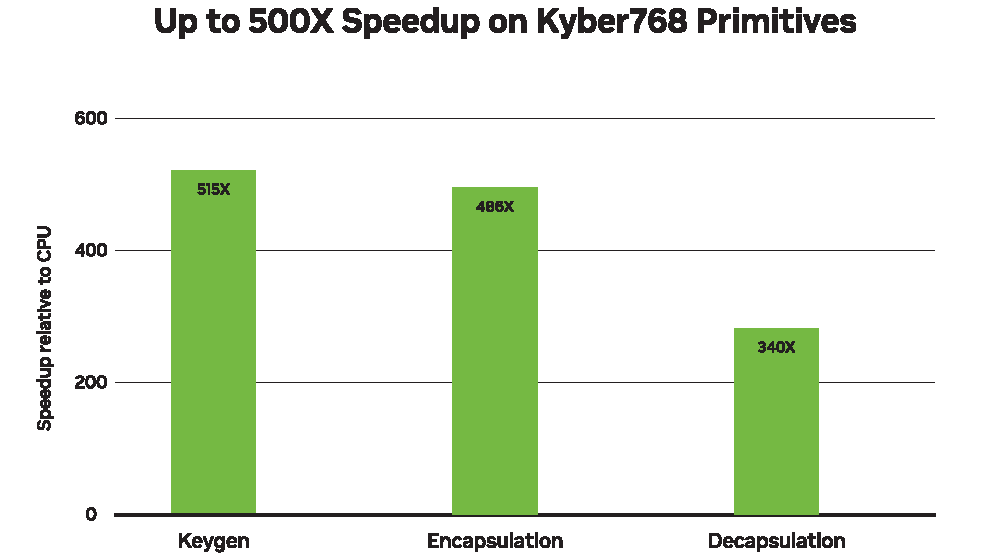
\includegraphics[width=0.7\linewidth]{images/quantum-computing-cupqc}
	\caption{Измерения на чипе NVIDIA H100. Сравнение с современными однопоточными процессорами, используемыми в тестовом пакете liboqs \cite{cuPQC}.}
	\label{fig:quantum-computing-cupqc}
\end{figure}
    
Недавнее сотрудничество компании QuSecure, лидера в сфере постквантовой криптографии, с компанией NVIDIA, привело к серьезным шагам в сторону адаптации GPGPU вычислителей для задач <<Постквантовой Эры>> \cite{cuPQC_Blog}. Одно из основных достижений в рамках сотрудничества -- создание CUDA cuPQC -- SDK (Software Development Kit) оптимизированных библиотек для ускорения передовых постквантовых алгоритмов. Заявляется $300-500x$ ускорение алгоритма Kyber 768 относительно оптимизированных с помощью Intel AVX реализаций (см. рис. \ref{fig:quantum-computing-cupqc}).  

\subsection{Квантовые решения}

На текущий момент существует два класса задач, которые успешно решаются существующими квантовыми решениями: генерация случайных чисел (ГСЧ) и квантовое распределение ключей.

\subsubsection{Генерация случайных чисел}

Важность генерации случайных чисел сложно переоценить. Случайные числа являются важнейшим ресурсом в огромном числе практических приложений. Последовательности случайных чисел применяются в системах безопасности, криптографии, в научных исследованиях (статистике, моделировании различных систем и процессов).

Генераторы случайных чисел традиционно делят на две категории: аппаратные (АГСЧ, англ. hardware random number generator, HRNG) и псевдослучайные (ПГСЧ, англ. pseudorandom number generator, PRNG).

Устройства, основанные на макроскопических случайных процессах, не могут обеспечить скорости получения случайных чисел, достаточной для прикладных задач. Поэтому в основе современных АГСЧ лежат источники шума, из которых извлекаются случайные биты: дробовой шум, радиоактивный распад, спонтанное параметрическое рассеяние \cite{Henk}.

Основная проблема аппаратных генераторов случайных чисел — это их относительно медленная по сравнению с генераторами псевдослучайных последовательностей работа. Также многие из них постепенно деградируют со временем, а анализ и верификация таких генераторов задача весьма затруднительная.

Квантовые генераторы случайных чисел (КГСЧ) в качестве физического источника энтропии используют квантовые процессы, которые сами по себе имеют вероятностную природу, что делает их идеально подходящими для криптографических приложений.

Решения Quantis QRNG Chip ветерана отрасли -- компании ID Quantique (IDQ), достигают скорости генерации $20 Mb/s$ \cite{Quantis_QRNG}. Не уступает им и ближайший конкурент Crypta Labs, предоставляя генераторы Firefly PCIe QRNG со скоростью генерации до $20 Mb/s$ \cite{CryptaLabs_Firefly}.

Если требуется высокая скорости генерации, то по этому критерию на порядок обходит конкурентов компания Quantum Dice со своими генераторами VERTEX 1100 \cite{QuantumDice_VERTEX} и APEX 2100 \cite{QuantumDice_APEX}, достигающими скорости генерации случайной последовательности бит $2.66 Gb/s$ и $7.5 Gb/s$ соответственно.

Активная работа по созданию передового КГСЧ сегодня ведется отечественной компанией QRate. Скорость их решения QRate Chaos будет превышать $1 Gb/s$ \cite{QRateChaos}.  


\subsubsection{Квантовое распределение ключей}

Генерация общего ключа является краеугольным камнем любой симметричной криптосистемы. Задача безопасной передачи с последующим хранением ключа обладает высочайшей сложностью. Всегда существует риск утраты конфиденциальности, связанный с компрометацией ключа, в том числе и неявной: увольнение сотрудника, который имел допуск к ключевой информации, необходимость допуска сотрудников других организаций и так далее. Чем дольше используется один и тот же ключ, тем выше вероятность того, что он уже явно или неявно скомпрометирован. Но помимо риска компрометации при длительном использовании одного и того же ключа существует ограничение на объем шифруемой информации. После исчерпания ключа, взлом можно попытаться осуществить статистическими методами.

\begin{figure}[h]
	\centering
	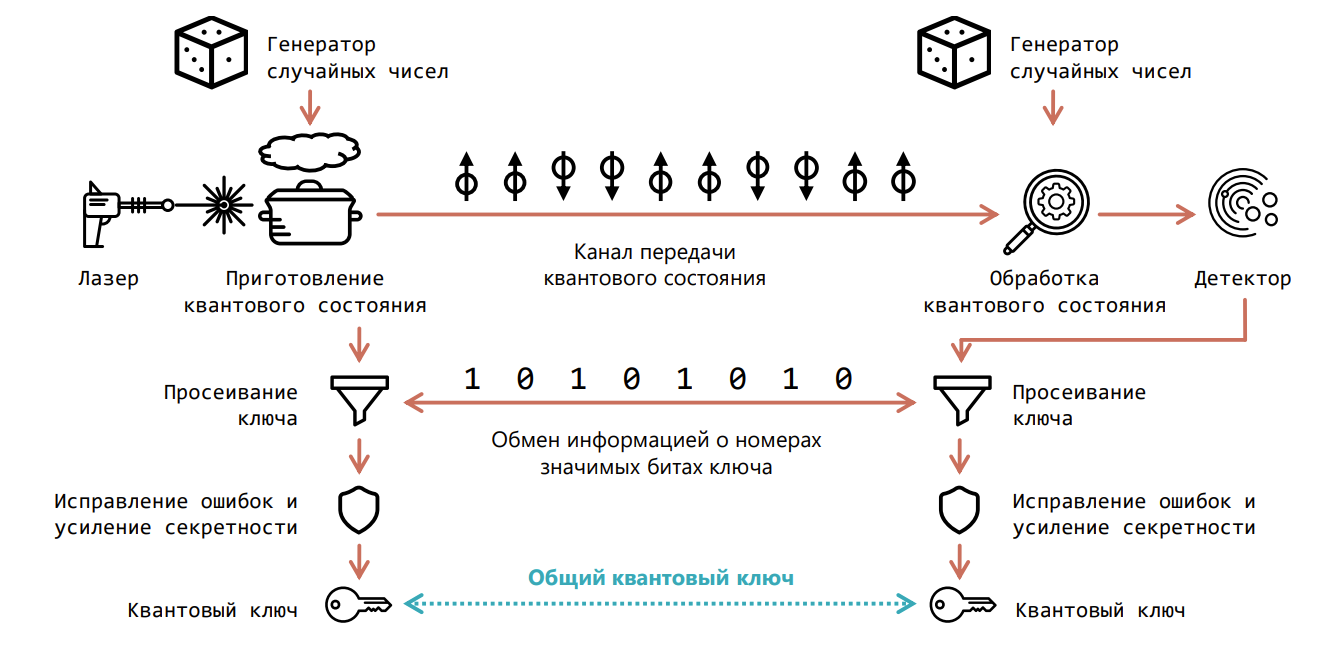
\includegraphics[width=0.7\linewidth]{images/infotecs_distrib}
	\caption{Квантовое распределение ключей. Принцип действия \cite{Infotecs_Sheet}.}
	\label{fig:infotecskeys}
\end{figure}


Предложенное Стивеном Визнером (англ. Stephen Wiesner) в 1983 г. решение проблемы генерации общего секрета, используя квантовые принципы, оказалось весьма удачным \cite{Stephen_Wiesner}. Последующая разработка привела к созданию алгоритмов квантового распределения ключей (КРК) — семейства криптографических протоколов, позволяющих двум удаленным абонентам выработать общий случайный секрет (ключ). 

Гарантия безопасности квантового распределения ключей заложена в протоколе фундаментально. Считается, что секретность выработки квантовых ключей основана на следующих принципах:

\begin{enumerate}
	\item Невозможно клонировать неизвестное квантовое состояние.
	\item Невозможно различить два неортогональных квантовых состояния.
	\item Невозможно измерить квантовое состояние без его изменения (редукция волновой функции).
\end{enumerate}

Эти принципы позволяют гарантированно детектировать пассивного/активного злоумышленника, что делает невозможным атаку <<человек по середине>>, другими словами незаметную компрометацию ключа шифрования.

Протокол КРК имеет ряд существенных преимуществ перед классическими протоколами передачи секрета: доказанная секретность квантовых ключей, отсутствие необходимости в постоянном администрировании, стойкость к криптографическим атакам с применением квантового компьютера, высокая скорость смены ключей.

Аппаратные решения, реализующие протокол квантового распределения ключей, являются типичными представителями класса усилителей, обеспечивая надежное создание криптографического ключа на узлах. Схема общепринятой организации протокола приведена на рисунке \ref{fig:infotecskeys}. 


В конце 2020 года компания <<ИнфоТеКС>> совместно с физическим факультетом МГУ имени М.В. Ломоносова представили лабораторные образцы ViPNet Quandor - коммерческого отечественного комплекса, работающего в топологии <<точка-точка>>, включающего аппаратуру для КРК \cite{Infotect_ViPNet1_MSU}. Современный приемник ViPNet Quandor 2, обладает скоростью выработки квантовых ключей 256 бит/мин с максимальной длиной квантового канала 100 км \cite{Infotect_ViPNet2}. Наращивание компетенций компании привело к созданию ViPNet Quantum Trusted System (ViPNet QTS) - решению для создания квантовой криптографической сети произвольной топологии \cite{Infotect_QTS}.

Компания ID Quantique (IDQ), лидер в области квантовой коммуникации, продает свои реализации протокола квантового распределения ключей. Передовое решение Clavis XG QKD System предлагает длину канала до 150 км с поддержкой произвольных топологий. Более приземленная аппаратура Cerberis XG QKD System обладает каналом до 90 км \cite{IDQ_QKD}. 

\section{Заключение}


В работе были определены основные причины использования аппаратных решений, акцент поставлен на применение в области защиты информации. Описана идея баланса процесса разработки аппаратуры в терминах PPA (Power, Performamce, Area).

Проведена классификация аппаратных решений для задач защиты информации - разбиение на два пересекающихся класса: усилители и ускорители.

Был проведен обзор существующих передовых решений в классе ускорителей: расширения центрального процессора (CPU) и графические процессоры общего назначения (GPGPU). 

Дано описание задач, эффективно решаемых квантовыми системами: квантовые генераторы случайных чисел и квантовое распределение ключей. Приведены актуальные аппаратные реализации квантовых протоколов.

За рамками данной работы осталась интересная область аппаратуры для защиты информации на основе программируемых логических интегральных схем (ПЛИС, англ. FPGA), которые обладают существенно укороченным циклом разработки, что приводит к разнообразию таких чипов.





\newpage
%\LaTeX{} \cite{latex2e} is a set of macros built atop \TeX{} \cite{texbook}.
\bibliographystyle{IEEEtran} % We choose the "plain" reference style
%\bibliography{IEEEabrv, refs} % Entries are in the refs.bib file
\bibliography{refs}


%https://www.cnbc.com/2024/06/02/nvidia-dominates-the-ai-chip-market-but-theres-rising-competition-.html
\end{document}



